%%%%%%%%%%%%%%%%%%%%%%%%%%%%%%%%%%%%%%%%%%%%%%%%%%%%%%%%%%%%%%%%%%%%%%%%%%%%%
%%%                              Fieldgroup                               %%%
%%%%%%%%%%%%%%%%%%%%%%%%%%%%%%%%%%%%%%%%%%%%%%%%%%%%%%%%%%%%%%%%%%%%%%%%%%%%%
\subsubsection{Fieldgroup}
\label{sec:uifieldgroup}
\input{diagrams/ui_fieldgroup_list}
\index{FIELDGROUP@\FIELDGROUP!ui\_manager fieldgroup}

Fieldgroups have a unique identifier and
consist of vertically aligned field lines separated by commas.
A field line has strings, text fields, option menus
or a pair of arrows to scroll the data items within a table.
It can also have many other gui elements (INDEX, LIST, TABLE, ...).
All fieldgroup items are placed left justified except items that are
followed by a \verb+'>'+ or a \verb+'|'+.

\input{diagrams/ui_fieldgroup_line}

\index{data item!fieldgroup}
\index{VOID@\VOID!fieldgroup}
\index{STRETCH@\STRETCH!fieldgroup}
\index{PIXMAP@\PIXMAP!fieldgroup}
\index{index identifier!fieldgroup (GUI index)}
\index{fieldgroup identifier!fieldgroup}
\index{thermo identifier!fieldgroup}
\index{list identifier!fieldgroup}
\index{table identifier!fieldgroup}
\index{plot2d identifier!fieldgroup}
\index{folder identifier!fieldgroup}
\index{SEPARATOR@\SEPARATOR!fieldgroup}
\index{ARROWS@\ARROWS!fieldgroup}
\index{environment var!APPHOME@\$APPHOME}
\index{environment var!BITMAP\_PATH@\$BITMAP\_PATH}
\begin{tabularx}{\textwidth}{l|X}
  line element & description  \\
  \hline
  {\verb+data reference+}        & display a data item
                                   (see section \nameref{dia:uifielddatareference}
                                    on page \pageref{dia:uifielddatareference}) \\
  {\verb+string+}                & creates a text label.\\
  \VOID                          & creates an empty space which can be used for alignment. \\
  \STRETCH                       & define stretch factors for the column and row.
                                   They make the column / row expand if additional space is available.
                                   A higher stretch factor expands more. \\
  \PIXMAP (string)               & Filename (with or without extension). \newline
                                   Displays a image. \newline
                                   File is searched in following directories: \newline
                                   \$BITMAP\_PATH : colon (linux) or semicolon (windows)
                                    separated list of directories \newline
                                   \$APPHOME/bitmaps \newline
                                   IntensHome/bitmaps : IntensHome is the parent directory of
                                   the \INTENS{} executable \newline
                                   ./bitmaps \newline
                                   . \\
  \PIXMAP (data\_reference)      & Datapool variable (\STRING{} or \CDATA). \newline
                                   The value of the variable can be a filename (with or without extension)
                                   of the image to display or the image itself (image file content). \newline
                                   If it is a filename, the file is searched in the directories as described above
                                   (\PIXMAP (string)). \\
  {\verb+ID_INDEX+}              & display an index object (see section \nameref{sec:uiindex} on page \pageref{sec:uiindex}) \\
  {\verb+ID_FIELDGROUP+}         & display a fieldgroup object (see section \nameref{sec:uifieldgroup} on page \pageref{sec:uifieldgroup}) \\
  {\verb+ID_THERMO+}             & display a thermo object (see section \nameref{sec:uithermo} on page \pageref{sec:uithermo}) \\
  {\verb+ID_LIST+}               & display a list object (see section \nameref{sec:uilist} on page \pageref{sec:uilist}) \\
  {\verb+ID_TABLE+}              & display a table object (see section \nameref{sec:uitable} on page \pageref{sec:uitable}) \\
  {\verb+ID_PLOT2D+}             & display a plot2d object (see section \nameref{sec:uiplot2d} on page \pageref{sec:uiplot2d}) \\
  {\verb+ID_FOLDER+}             & display a folder (see section \nameref{sec:uifolder} on page \pageref{sec:uifolder}) \\
  \SEPARATOR                     & creates a horizontal (default) or vertical separator \newline
                                   To create a vertical separator, add the option \VERTICAL. \newline
                                   To create a vertical separator over multiple rows, add the option \ROWSPAN = n. \newline
                                   The vertical separator can be left (default), center or right aligned (within the column). \newline
                                   Example: centered vertical separator, two rows high: \newline
                                   \SEPARATOR | \{\VERTICAL, \ROWSPAN=2\} \\
  \ARROWS                         & inserts a row/column with an additional index (to scroll the table elements) and
                                    row/column header. \newline
                                   Only allowed in tables. (Fieldgroup must have \TABLESIZE{} set.) \\
\end{tabularx}

\input{diagrams/ui_field_additional_attributes}

\index{PIXMAP@\PIXMAP!fieldgroup}
\index{SIZE@\SIZE!fieldgroup}
\index{SCROLLBARS@\SCROLLBARS!fieldgroup}
\index{AUTO\_SCROLL@\AUTOSCROLL!fieldgroup}
\index{EXPAND@\EXPAND!fieldgroup}
\index{COLSPAN@\COLSPAN!fieldgroup}
\index{ROWSPAN@\ROWSPAN!fieldgroup}
\index{VERTICAL@\VERTICAL!fieldgroup}
\index{ROTATE\_180@\ROTATEONEEIGHTY!fieldgroup}
\index{HELPTEXT@\HELPTEXT!fieldgroup}
\index{CLASS@\CLASS!fieldgroup}
\begin{tabularx}{\textwidth}{l|X}
  attribute     & description  \\
  \hline
\verb+string+   & TODO \\
\PIXMAP         & display button-items picture faced \\
\SIZE (w, h)    & scale the \PIXMAP{} to this size (in pixel) \\
\SCROLLBARS     & attach a scrollbar to the multiline textfield \\
\AUTOSCROLL     & automatically scroll to the end of the multiline textfield \\
\EXPAND         & make field expandable \\
\COLSPAN{} = n  & ui field uses n columns \\
\ROWSPAN{} = n  & ui field uses n rows \\
\VERTICAL       & draw ui field vertically \\
\ROTATEONEEIGHTY  & draw ui field rotated 180 degrees \\
\HELPTEXT       & use the given \STREAM{} as the \HELPTEXT{} of the field \\
\CLASS          & set \CLASS{} property of the field (used in qt style sheets) \\
\end{tabularx}

\newpage
Example: \\

\begin{boxedminipage}[t]{\linewidth}
\begin{alltt}
\DESCRIPTION "Example PIXMAP";
\DATAPOOL
  \SET
    pixmap_set ("plot2d", "semafor-logo");
  \STRING \{EDITABLE\}
    filename \{\SET = pixmap_set\};
\END \DATAPOOL;

\UIMANAGER
  \FIELDGROUP
    Group_1 (
        filename \PIXMAP( filename, 100, 50 )
      )
   ;
  \FORM
    Form_1
      ( ( Group_1 )
      )
   ;
\END \UIMANAGER;
\END.
\end{alltt}
\end{boxedminipage}


\vspace{0.5cm}

\input{diagrams/ui_field_alignment}
\input{diagrams/ui_field_void_size}

\index{justify!fieldgroup}
\index{  @Signs / Characters!\texttt{"<} (less than)!justify}
\index{  @Signs / Characters!\texttt{">} (greater than)!justify}
\index{  @Signs / Characters!\texttt{"|} (vertical line)!justify}
\index{  @Signs / Characters!\% (percent)!relative void size}

\begin{tabularx}{\textwidth}{l|X}
alignment           & description \\ \hline
{\bfseries $<$}     & the field is right aligned (within the column) \\
{\bfseries $>$}     & the field is left aligned (within the column) \\
{\bfseries $\mid$}  & the field is centered (within the column) \\
{\bfseries $\^$}  & the field is top aligned (within the row) \\
{\bfseries $\_$}  & the field is bottom alligned (within the row) \\ \hline
void size           & minimal width, height of the field \newline
                      w, h in pixels or relative to form size (\%) \\
\end{tabularx}

\input{diagrams/ui_field_pixmap_size}

\begin{tabularx}{\textwidth}{l|X}
pixmap field size   & description \\ \hline
empty               & size of the image is used \\
, x, y              & size in pixels the image is scaled to \\
\end{tabularx}

\input{diagrams/ui_field_options}
\index{COLSPAN@\COLSPAN!fieldgroup field option}
\index{ROWSPAN@\ROWSPAN!fieldgroup field option}
\index{VERTICAL@\VERTICAL!fieldgroup field option}
\index{ROTATE\_180@\ROTATEONEEIGHTY!fieldgroup}
\index{HELPTEXT@\HELPTEXT!fieldgroup}
\index{CLASS@\CLASS!fieldgroup}

\begin{tabularx}{\textwidth}{l|X}
option              & description \\ \hline
\COLSPAN{} = n      & ui field uses n columns \\
\ROWSPAN{} = n      & ui field uses n rows \\
\VERTICAL           & draw ui field vertically \\
\ROTATEONEEIGHTY    & draw ui field rotated 180 degrees \\
\HELPTEXT           & use the given \STREAM{} as the \HELPTEXT{} of the field \\
\CLASS              & set \CLASS{} property of the field (used in qt style sheets) \\
\end{tabularx}
\vspace{0.5cm}

The value displayed in the textfield is the value of the
data item (optionally multiplied by a scale factor) referenced by the
identifier.

Text fields have a default width of 8 characters. It can be changed
providing a ui\_field\_length. The first integer (after the :) is the
width, the optional second integer is the precision.
If the width is a negative integer value, the alignment of the value within the field
is inverted: strings are left aligned (default is right), numbers are right aligned
(default is left).
The precision specifies the number of lines for a string or the number
of digits after the decimal point for a real number.

Examples:
\begin{itemize}
\item \verb+s:50:3+ \newline
      \STRING{} s in a text area 50 characters wide and 3 high
\item \verb+r*1e3:-12:3:TSEP+ with r = 12.3456789 \newline
      |12'345.679  | \newline
      value of \REAL{} r multiplied by 1000, value is left aligned,
      field width is 12 characters, precision 3,
      thousand separator is shown
\end{itemize}

\input{diagrams/ui_field_attributes}
\input{diagrams/ui_field_length}
\label{sec:uifieldlength}
\input{diagrams/ui_field_precision}
\label{sec:uifieldprecision}
\index{data item!ui field attributes}
\index{data item!ui field length}
\index{data item!ui field precision}

\index{  @Signs / Characters!- (hyphen)!left alignment}
\index{  @Signs / Characters!- (hyphen)!right alignment}
\index{  @Signs / Characters!: (colon)!dataitem-format width}
\index{  @Signs / Characters!: (colon)!dataitem-format precision}
\index{  @Signs / Characters!: (colon)!dataitem-format tsep}
\index{Scale factors!dataitem-format}
\index{width}
\index{precision}
\index{TSEP@\TSEP!dataitem-format}
\index{String!multiple lines (precision)}
\begin{tabularx}{\textwidth}{l|X}
data item format   & description \\
\hline
\verb+scale+       & see section \nameref{sec:scale} page \pageref{sec:scale} \\
                   & defines the factor that multiplies the items
                    value before displaying and the divisor that divides
                    the input value before saving in the datapool. \newline
                    (has no meaning for STRING items) \\
{\verb+-+}         & Alignment: inverses the alignment \\
                   & a) alignes the \STRING{} data item to the right (default is left) \\
                   & b) alignes the numeric data item to the left (default is right) \\
{\verb+width+}     & defines the length of the field \\
                    & a) only that many characters can be entered for numeric items,\\
                    & b) more characters can be entered for \STRING{} items\\
{\verb+precision+} & a) defines the number of digits after the decimal point for \REAL{} items,\\
                   & b) defines the number of lines for \STRING{} items\\
\TSEP              & Thousand separator (12{\bfseries '}345.67) (for \REAL{} items only). \\
\end{tabularx}

\newpage
\input{diagrams/ui_fieldgroup_options}
\input{diagrams/ui_fieldgroup_option}
\label{sec:uifieldgroupotions}

The FIELDGROUP options define the behaviour and appearance of the fieldgroup.

\index{JUSTLEFT@\JUSTLEFT!fieldgroup option}
\index{JUSTRIGHT@\JUSTRIGHT!fieldgroup option}
\index{CENTER@\CENTER!fieldgroup option}
\index{TABLESIZE@\TABLESIZE!fieldgroup option}
\index{STEP@\STEP!fieldgroup option}
\index{ORIENTATION@\ORIENTATION!fieldgroup option}
\index{NAVIGATION@\NAVIGATION!fieldgroup option}
\index{HORIZONTAL@\HORIZONTAL!fieldgroup option}
\index{VERTICAL@\VERTICAL!fieldgroup option}
\index{POSITION@\POSITION!fieldgroup option}
\index{RANGE@\RANGE!fieldgroup option}
\index{MENU@\MENU!UI\_MANAGER!FIELDGROUP MENU=HIDDEN}
\index{HIDDEN@\HIDDEN!fieldgroup option \MENU=\HIDDEN}
\index{ARROWS@\ARROWS!fieldgroup option \ARROWS=\HIDDEN}
\index{HIDDEN@\HIDDEN!fieldgroup option \ARROWS=\HIDDEN}
%%(not implemented in intens-qt) \index{ALIGN@\ALIGN!fieldgroup option}
\index{FRAME@\FRAME!fieldgroup option}
\index{MARGIN@\MARGIN!fieldgroup option}
%%(not implemented in intens-qt) \index{JUSTIFY@\JUSTIFY!fieldgroup option}
\index{INDEX@\INDEX!fieldgroup option}
\index{CLASS@\CLASS!fieldgroup option}
\begin{tabularx}{\textwidth}{l|X}
option              & description \\
\hline
{\verb+string+}     & The title of the fieldgroup \\
\JUSTLEFT           & \\
\JUSTRIGHT          & \\
\CENTER             & Without one of these options, \INTENS{} places the table fields left
                      justified within each column. \\
\TABLESIZE          & creates a table with arrow buttons to scroll
                      through the items. There is only one
                      {\verb+data_item+} per line allowed. \\
\STEP               & defines the step width that is scrolled with one
                      arrow click. \\
\STEP{} = 0         & no scrolling is possible (the arrow buttons are not created) \\
\ORIENTATION        & The tables default orientation is \HORIZONTAL. \\
\NAVIGATION         & determines the direction in which the tables
                      text fields are to be traversed during keyboard navigation.
                      \HORIZONTAL{} is the default value. \\
\POSITION = n       & defines which element is shown multiple times. \newline
                      n = 2 would show the first two elements (0 and 1) once and the
                      third element (index 2) multiple times. \newline
                      {\bfseries 1} is the default value. \\
\RANGE              & determines the index range that can be used
                      for the associated data items. The default starting index is 0. \\
\MENU=\HIDDEN       & Do not display table row/column menu, when right mouse button is pressed at row/column header. \newline
                      Is used in conjunction with option \TABLESIZE. \\
\ARROWS=\HIDDEN     & Do not display table row/column header. \newline
                      Is used in conjunction with option \TABLESIZE. \\
%%(not implemented in intens-qt) \ALIGN              & TODO \\
\FRAME              & Display a frame around the fieldgroup \\
\MARGIN             & Set margin (and optionally spacing) in pixels \\
%%(not implemented in intens-qt) \JUSTIFY            & TODO \\
\INDEX=ID\_INDEX    & Use an \INDEX{} object (see section \nameref{sec:uiindex}
                      on page \pageref{sec:uiindex}) as the \INDEX{} of the \FIELDGROUP. \newline
                      This makes it possible to set and read the value of
                      the \FIELDGROUP{} \INDEX{}. \newline
                      Is used in conjunction with option \TABLESIZE. \\
\CLASS               & set \CLASS{} property of the \FIELDGROUP{} (used in qt style sheets) \\
\end{tabularx}
%

%---------------------------------------------------------------------------%
%                                 Examples                                  %
%---------------------------------------------------------------------------%
\newpage

\begin{figure}\label{fig:fieldgroup1}
   \begin{center}
      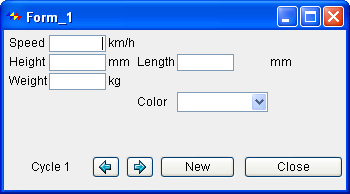
\includegraphics[width=0.6\linewidth]{grab_fieldgroup1}
   \end{center}
\caption{Example without FIELDGROUP options}
\end{figure}

\paragraph{Fieldgroup Examples}
%\subsubsection{Fieldgroup Examples}
\label{sec:uifgexamples}
The following examples show various configuration options of the fieldgroup.

The configuration 'Example 1' uses no fieldgroup options.
\INTENS{} places all fields left justified
(see page \pageref{fig:fieldgroup1}).


\begin{boxedminipage}[t]{\linewidth}
\begin{alltt}
\DESCRIPTION "Example 1";
\DATAPOOL
  \SET
     Colors ("red" = 1,"green" = 2,"blue" = 3)
    ;
  \REAL \{\EDITABLE\}
    speed ,height ,length ,weight
  ;
  \INTEGER \{\EDITABLE\}
    color \{\SET = Colors\}
  ;
\END \DATAPOOL;

\UIMANAGER
  \FIELDGROUP
    Group_1
      ( "Speed"    speed   "km/h"
      , "Height"   height  "mm"   "Length"   length  "mm"
      , "Weight"   weight  "kg"
      , \VOID       \VOID    \VOID    "Color"    color
      )
   ;
  \FORM
    Form_1
      ( ( Group_1 )
      )
   ;
\END \UIMANAGER;
\END.
\end{alltt}
\end{boxedminipage}


%---------------------------------------------------------------------------%
\newpage

\begin{figure}\label{fig:fieldgroup2}
   \begin{center}
      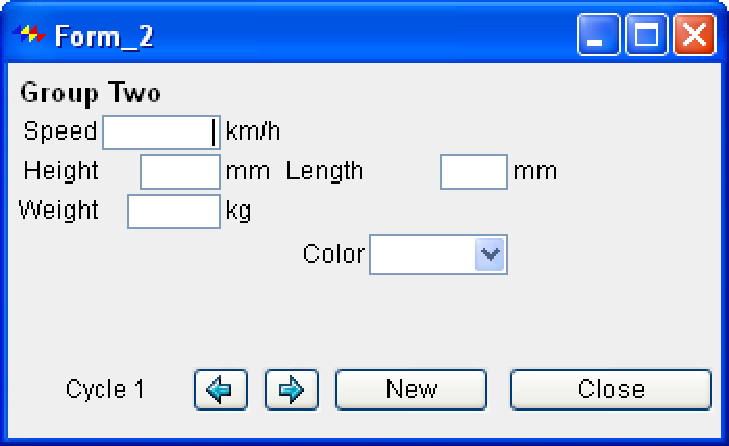
\includegraphics[width=0.6\linewidth]{grab_fieldgroup2}
   \end{center}
\caption{Example with option \JUSTRIGHT{} and fieldgroup title}
\end{figure}

The second example uses the option \JUSTRIGHT{} and sets the fieldgroup
\index{JUSTRIGHT@\JUSTRIGHT!fieldgroup option!example}
title ``Group Two''. All fields except those with a following '\verb+<+' character
are right justified within the fieldgroup.
(see page \pageref{fig:fieldgroup2}).


\begin{boxedminipage}[t]{\linewidth}
\begin{alltt}
\DESCRIPTION "Example 2";
\DATAPOOL
  \SET
    color_set ("red" = 1, "green" = 2, "blue" = 3 )
  ;
  \REAL \{\EDITABLE\}
    speed, height, length, weight
  ;
  \INTEGER \{\EDITABLE\}
    color \{ \LABEL="Color:", \SET=color_set \}
  ;
\END \DATAPOOL;

\UIMANAGER
  \FIELDGROUP
    Group_2 \{"Group Two", \JUSTRIGHT\} (
      "Speed:">  speed*3.6>       "km/h"<
    , "Height:"> height:5:1>      "m"<    "Length:"> length:4> "m"<
    , "Weight:"> weight*1e-3:6:2> "kg"<   \VOID      \VOID     \VOID
    , \VOID      \VOID            \VOID   "Color:">  color:5>  \VOID
    )
  ;
  \FORM
    Form_2
      ( ( Group_2 )
      )
   ;
\END \UIMANAGER;
\END.
\end{alltt}
\end{boxedminipage}


%---------------------------------------------------------------------------%
\newpage

\begin{figure}\label{fig:fieldgroup3}
   \begin{center}
      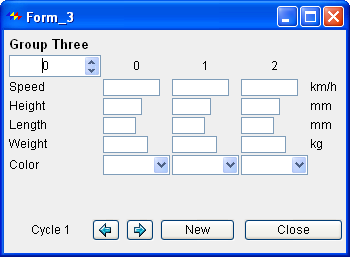
\includegraphics[width=0.6\linewidth]{grab_fieldgroup3}
   \end{center}
\caption{example with the option TABLESIZE=3}
\end{figure}

The third example shows data items arranged as a table.
This is done with the option \TABLESIZE{}.


\begin{boxedminipage}[t]{\linewidth}
\begin{alltt}
\DESCRIPTION "Example 3";
\DATAPOOL
  \SET
     Colors ("red" = 1,"green" = 2,"blue" = 3)
    ;
  \REAL \{\EDITABLE\}
    speed ,height ,length ,weight
  ;
  \INTEGER \{\EDITABLE\}
    color \{\SET = Colors\}
  ;
\END \DATAPOOL;

\UIMANAGER
  \FIELDGROUP
    Group_3 \{"Group Three", \TABLESIZE = 3 \STEP 2\}
      ( "Speed"    speed       "km/h"<
      , "Height"   height:5:1  "mm"<
      , "Length"   length:4    "mm"<
      , "Weight"   weight:6:2  "kg"<
      , "Color"    color:5
      )
   ;
  \FORM
    Form_3
      ( ( Group_3 )
      )
   ;
\END \UIMANAGER;
\END.
\end{alltt}
\end{boxedminipage}
